\documentclass[10pt,frenchb]{beamer}

\usepackage[utf8]{inputenc}
\usetheme[progressbar=frametitle]{Copenhagen} 
\usepackage{appendixnumberbeamer}

\usepackage{graphicx}
\usepackage{wrapfig}
\usepackage{xcolor}            
\usepackage{booktabs}
\usepackage{amsmath}
\usepackage{amssymb}
\usepackage[scale=2]{ccicons}

\usepackage{pgfplots}
\usepgfplotslibrary{dateplot}

\usefonttheme{professionalfonts}
\usepackage{times}
\usepackage{tikz}
\usepackage{amsmath,amssymb}
\usepackage{verbatim}
\usepackage{algorithm,algorithmic}
\usepackage{url}
\usetikzlibrary{arrows,shapes}	
\pgfplotsset{compat=1.4}

\DeclareMathOperator*{\argmax}{arg\,max\,}
\DeclareMathOperator*{\argmin}{arg\,min\,}

\author{Cl\'{e}mence R\'{e}da}
\title[Recommender system with serendipity]{\textbf{Graphs in ML Project Defence}\\
Recommender system with serendipity}
\institute{\'{E}cole Normale Sup\'{e}rieure Paris-Saclay}
\date{January $17^{\text{th}}$, 2019}

\makeatletter
\let\ALG@name\@empty% hack package algorithm
\let\fnum@algorithm\fname@algorithm% hack package float
\makeatother

\newlength\myindent
\setlength\myindent{2em}
\newcommand\bindent{%
  \begingroup
  \setlength{\itemindent}{\myindent}
  \addtolength{\algorithmicindent}{\myindent}
}
\newcommand\eindent{\endgroup}
 
\begin{document}
\maketitle

% 15''
%Reusing material / figures / slides from other people. You can take figures from papers or other people’s slides to illustrate an algorithm or explain a method. However, always properly acknowledge the source if you do so.

\section{Introduction}

\subsection{Field of research}

\begin{frame}
\frametitle{\textbf{Introduction} Field of research}

\begin{center}\end{center}

\begin{columns}
\begin{column}{0.7\textwidth}
\begin{center}
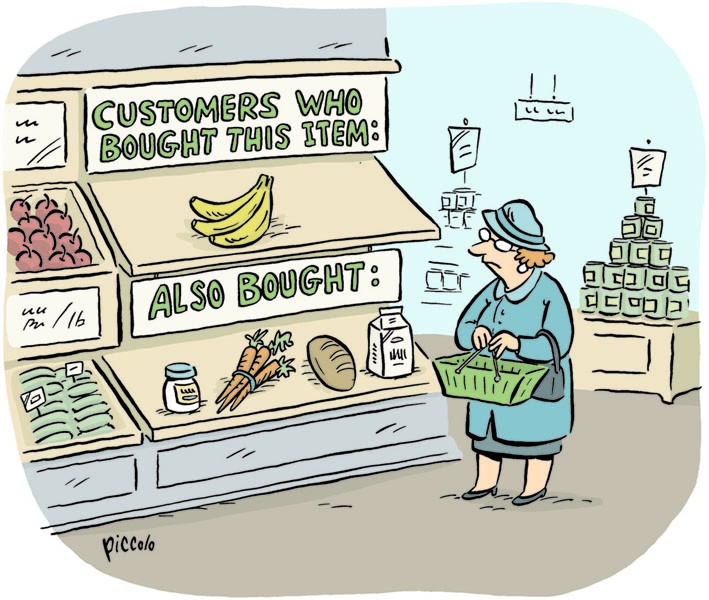
\includegraphics[height=125px]{images/recommender.jpeg}
\end{center}
\begin{center}\textit{Comic from artist Piccolo}\end{center}
\end{column}

\begin{column}{0.3\textwidth}
\begin{center}\textbf{This might be a useful recommender system!}\end{center}
\end{column}
\end{columns}

\end{frame}

\begin{frame}
\frametitle{\textbf{Introduction} Field of research}

\begin{center}\end{center}

\begin{columns}
\begin{column}{0.7\textwidth}
\begin{center}
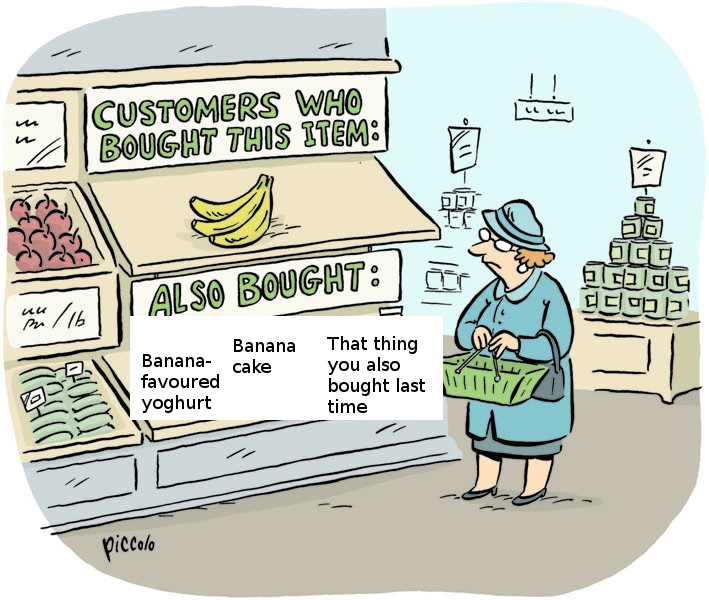
\includegraphics[height=125px]{images/recommender2.jpeg}
\end{center}
\begin{center}\textit{(Adapted) comic from artist Piccolo}\end{center}
\end{column}

\begin{column}{0.3\textwidth}
\begin{center}\textbf{This might be a \underline{useless} recommender system!}\end{center}
\end{column}
\end{columns}

\end{frame}

\begin{frame}{\textbf{Outlines}}
\tableofcontents
\end{frame}

 \begin{frame}
 \tableofcontents[currentsection]
 \end{frame}

\begin{frame}
\frametitle{\textbf{Introduction} Field of research}

\begin{center}\textbf{Accuracy $\neq$ Usefulness!}\\
\cite{abbassi2009getting,kunaver2017diversity}, ...
\end{center}
 
% accurate recommendations (that is, the user actually enjoys the recommended item, and buys it or rates it positively)

\begin{block}{Regular recommender problem}
\textbf{Input}:
\begin{itemize}
\item A user $u$
\item A set of objects $V$ in which the recommended item must belong
\item Access to the histories of the user(s): $\{(\text{object}_k, \text{reward}_k)\}_{k}$
\end{itemize}
\textbf{Goal}: 
\begin{center}Return a recommended item\\that maximizes the reward for the seller\\(price, probability of buying, ...)\end{center}
\end{block}

\end{frame}

\begin{frame}
\frametitle{\textbf{Introduction} Field of research}

\begin{center}\textbf{Accuracy $\neq$ Usefulness!}\\
\cite{abbassi2009getting,kunaver2017diversity}, ...
\end{center}
 
% useful recommendations (recommended items which are novelties, discoveries to the user things that they would never had found themselves)
%Serendipities are objects that are unexpectedly enjoyable. Two users’ reaction to a same recommended item can be poles apart.

\begin{block}{Recommender problem \textbf{with serendipity}}
\textbf{Input}:
\begin{itemize}
\item A user $u$
\item A set of objects $V$ in which the recommended item must belong
\item Access to the histories of the user(s): $\{(\text{object}_k, \text{reward}_k)\}_{k}$
\end{itemize}
\textbf{Goal}: 
\begin{center}Return a recommended item\\that maximizes \textbf{both the reward}\\\textbf{and the novelness}.\end{center}
\end{block}

\end{frame}

\begin{frame}
\frametitle{\textbf{Introduction} Field of research}

\begin{center} $\thicksim$ \emph{diversity-accuracy dilemma} \cite{zhou2010solving}\\
$\rightarrow$ \emph{exploration-exploitation dilemma} in bandits\end{center}

\begin{center}
Bandits are popular tools to tackle the recommender problem \cite{koutrika2018recent,mary2015bandits,guillou2016large}.
\end{center}

\begin{algorithm}[H]
\caption{Multi-Armed Bandit}
\begin{algorithmic}[1]
\STATE Initialize scores associated with each action (\emph{eg} movie)
\STATE Repeat
\bindent
\STATE Compute the score of each action
\STATE Select the arm/action which maximizes the score
\STATE Receive the reward and improve the computation of the score
\eindent
\RETURN the arm associated with the highest score
\end{algorithmic}
\end{algorithm}

\end{frame}

\subsection{Goal}

\begin{frame}{\textbf{Introduction} Objectives of this project}

\begin{alertblock}{Goals}
\bigskip

\begin{enumerate}
\item Formalize the problem of \textbf{recommendation with serendipity}
\pause
\item Find a method to tackle this problem
\pause
\item Compare it with other bandit methods
\end{enumerate}
\bigskip

\end{alertblock}

%In this project, we will adapt a multi-armed bandit method for Online Influence Maximization to the problem of recommendation with serendipity, and analyze the results with respect to accuracy and diversity.

\end{frame}

\section{Problem of Serendipity}

 \begin{frame}
 \tableofcontents[currentsection]
 \end{frame}

\subsection{State-of-the-art}

\begin{frame}{\textbf{State-of-the-art}} 

\begin{center}
\textbf{Several definitions of \emph{serendipity}}\\
\cite{abbassi2009getting,murakami2007metrics,iaquinta2008introducing,kotkov2016survey}
\end{center}
\pause

What one would need:

\begin{center}
\begin{itemize}
\item A flexible definition %ie should not rely on the use of one's method
\item Easy to understand and grasp %ie not "far-fetched" parametrization
\item Should fit as much as possible the concept of serendipity %!= method with diversity
\end{itemize}
\end{center}

\end{frame}

\subsection{Formalization of the problem}

\begin{frame}{\textbf{Formalization}} 

\begin{itemize}
\item $\mathscr{G}(V, E)$ unweighted, undirected object similarity graph
% which is accessible and computable at start time, because, in the recommender setting, the set of objects is fixed and their feature vectors are known
\item Histories of the user $\{(\text{object}_k, \text{reward}_k)\}_{k}$
\bigskip

\begin{center} $f^{(k)}_u = \text{explored objects up to time }k$\\
 $r^{(k)}_u = \text{associated reward received up to time }k$\\
(\emph{random variables})
\end{center}
\end{itemize}
\bigskip

\begin{block}{Serendipity value}
\textbf{serendipity value} of an unexplored object $v$ (of \emph{normalized} reward variable $\~{r}̂^{(k)}_{v,u}$) at time $k > 0$ with respect to user $u$\\
\bigskip
\begin{center}
$s(v, u, k) = \mathbb{E}_{(f^{(k)}_u, \~{r}̂^{(k)}_u)}[\~{r}̂^{(k)}_{v,u} \times d_e(v, \text{explored})|(f^{(t)}_u, \~{r}̂^{(t)}_u)_{t < k}]$
\end{center}

\end{block}

% d e is the distance measure of the length (in number of edges) of the shortest path

\end{frame}

\begin{frame}{\textbf{Formalization}}

\begin{block}{Serendipity value}
\textbf{serendipity value} of an unexplored object $v$ (of \emph{normalized} reward variable $\~{r}̂^{(k)}_{v,u}$) at time $k > 0$ with respect to user $u$\\
\bigskip
\begin{center}
$s(v, u, k) = \mathbb{E}_{(f^{(k)}_u, \~{r}̂^{(k)}_u)}[\~{r}̂^{(k)}_{v,u} \times d_e(v, \text{explored})|(f^{(t)}_u, \~{r}̂^{(t)}_u)_{t < k}]$
\end{center}

\end{block}

Thus the set of potential serendipities at time $k > 0$ for user $u$ is denoted $\mathscr{S}_u$

\begin{alertblock}{Potential Serendipities}
\begin{center}
$\mathscr{S}_u = \argmax \{v \text{ unexplored} : s(v, u, k) \}$
\end{center}
\end{alertblock}

\end{frame}

\subsection{Method}

\begin{frame}{\textbf{Method} Adapting from Influence Maximization}

% Intuitively, what I want is to increase as fast as possible the support of f u while maximizing the expected rewards of objects in the support. This problem remotely looks like Influence Maximization

\begin{columns}
\begin{column}{0.6\textwidth}
\begin{center}
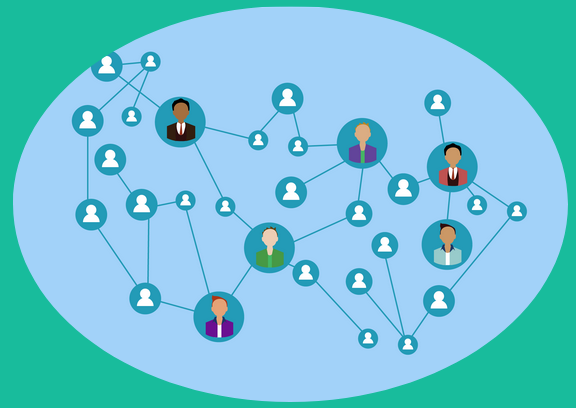
\includegraphics[height=125px]{images/influence.png}
\end{center}
\begin{center}\url{richardkim.me/influencemaximization}\end{center}
\end{column}

\begin{column}{0.4\textwidth}
\begin{center}To whom should products be given in order to become viral?\end{center}
\pause
\textbf{Online}: Learning while running the marketing campaign\\
\bigskip
\pause
\textbf{Persistent}: Once a node is explored, it does not yield a reward anymore
\end{column}
\end{columns}

\end{frame}

\begin{frame}{\textbf{Method} Algorithm from \cite{lagree2017effective}}

\textbf{Score}:
\begin{center}
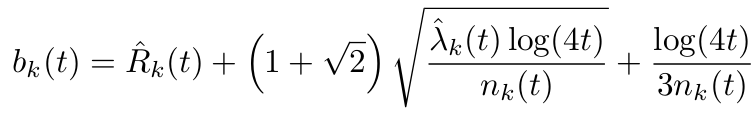
\includegraphics[height=30px]{images/score.png}\\
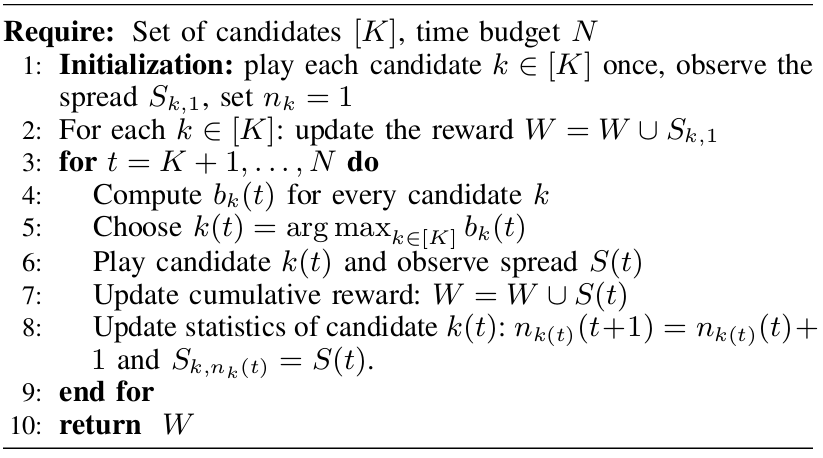
\includegraphics[height=150px]{images/gt-ucb.png}
\end{center}

\end{frame}

\begin{frame}{\textbf{Method} Adapted algorithm}

% -I want to select the candidates which will give the highest expected spread, the notion of spread here being the mix between reward and novelty defined in the definition of serendipity. 
\begin{block}{}
\begin{center}
Apply the serendipity constraint on the set of candidates\\(and their supports) selected in \cite{lagree2017effective}'s algorithm,\\parametrized by value $s$.
\end{center}
\end{block}

%$K$: number of candidates in which the recommended item should be selected, $s$: serendipity threshold, $W$: (unweighted, undirected) similarity graph matrix, $n$: total number of objects, $f$: number of features, $F$: object feature matrix of size $n \times f$

\begin{algorithmic}[1]
\STATE $S \leftarrow \text{Supp}(f^{(t)}_{u}) \cap \{c \in V : \exists i, 1 \leq i \leq s, W^{i}[c, \text{Supp}(f^{(t)}_{u})]\textbf{1} > 0 \}$
\STATE $\text{centroids} \leftarrow \text{Kmeans}(\text{data}=F[S,:],\text{nclusters}=K)$
\STATE $\text{candidates} \leftarrow \emptyset$
\FOR{$c \in \text{centroids}$}
\STATE Append $\argmin_{\substack{v \in S}} ||F[v, :]-F[c, :]||^{2}_2$ to $\text{candidates}$
\ENDFOR
\STATE $\text{supports} \leftarrow \emptyset$
\FOR{$v \in \text{candidates}$}
\STATE Append $\{v' \in S : W[v,v'] > 0\}$ to $\text{supports}$
\ENDFOR
\RETURN candidates, supports
\end{algorithmic}

\end{frame}

\section{Results}

 \begin{frame}
 \tableofcontents[currentsection]
 \end{frame}

\subsection{Datasets}

\begin{frame}{\textit{MovieLens}}

\textbf{Movie recommendation!} data on users, movies, and ratings\\
\begin{center}
(\textit{GroupLens Research}: \url{movielens.org})
\end{center}

\begin{center}
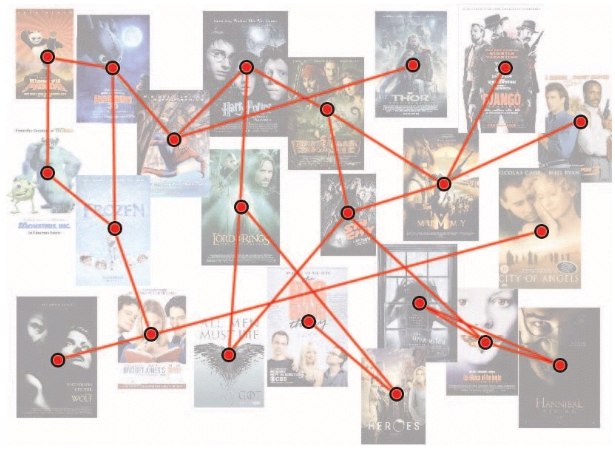
\includegraphics[height=130px]{images/movielens.png}
\end{center}
\begin{center}
\textit{M. Valko's slides for Lecture 7}
\end{center}

\end{frame}

\begin{frame}{\textit{MovieLens} (ml-1m, ml-20m)}

\begin{center}
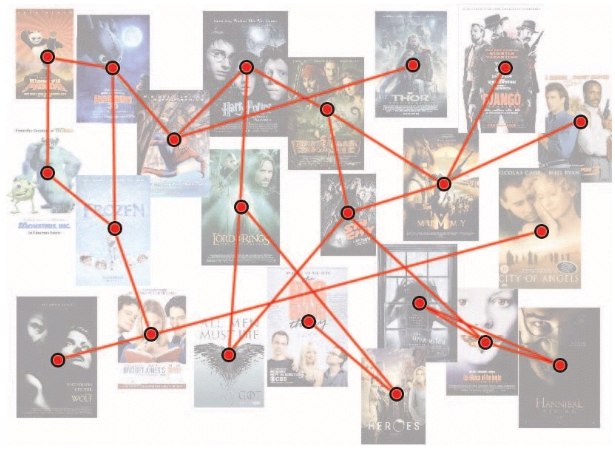
\includegraphics[height=50px]{images/movielens.png}
\end{center}

\begin{itemize}
\item \textbf{MovieLens 1M Dataset (ml-1m)}\\

\begin{table}
\begin{tabular}{|c|c|c|}
\hline
\textbf{\#movies} & \textbf{\#users} & \textbf{average \#ratings/user}\\
\hline
4,000 & 6,000 & 165\\
\hline
\end{tabular}
\end{table}

\item \textbf{MovieLens 20M Dataset (ml-20m)}\\

\begin{table}
\begin{tabular}{|c|c|c|}
\hline
\textbf{\#movies} & \textbf{\#users} & \textbf{average \#ratings/user}\\
\hline
27,000 & 138,000 & 144\\
\hline
\end{tabular}
\end{table}

\end{itemize}

\end{frame}

\subsection{Setting}

\begin{frame}{Benchmark on \textit{MovieLens} (ml-1m, ml-20m)}

\textbf{Evaluation} on $100$ iterations and at horizon $100$

\begin{block}{Cumulative regret}
$a^{(t)}$ is the recommended item at time $t$:
\begin{center}
$R_{T} & = \sum_{t \leq T} \text{max} \{ a^{*} \text{explored} : r(a^{*}) - r(a^{(t)}) \}$
\end{center}
\end{block}

%When computing the regret for the adapted version of Lagrée et al. [2017]’s method, we also assume that the best arm we could use is among the K selected candidates, thus that we do not challenge the candidate selection method, which is an hypothesis made in the original article.

\pause

\begin{block}{Diversity measure (\cite{vie2016modeles})}
$t$ is the number of rounds, $V^{(t)}$ is the feature matrix of explored objects up to time $t$
\begin{center}
$D(V^{(t)}) & = \sqrt{|V^{(t)}.t(V^{(t)})|}$
\end{center}
\end{block}

%The diversity measure defined in Equation 1. This volume should increase more for recommendation with serendipity than for regular recommendation, because recommended objects are supposed to be less correlated.

\end{frame}

\begin{frame}{Benchmark on \textit{MovieLens} (ml-1m, ml-20m)}

\textbf{Algorithms}

%Algorithms tested

\begin{alertblock}{Tested bandit methods}
\begin{enumerate}
\item Random strategy
\pause
\item $\epsilon$-greedy strategy (w.r.t. diversity measure)
\pause
\item LinUCB (described in \cite{chu2011contextual})
\pause
\item The adapted method from \cite{lagree2017effective}
\end{enumerate}
\end{alertblock}

\end{frame}

\subsection{Quantitative Results}

\begin{frame}{\textbf{Results} Regret, diversity, serendipity curves}

\textbf{ml-20m} dataset, random (\emph{top}) and $\epsilon$-greedy methods

\begin{center}
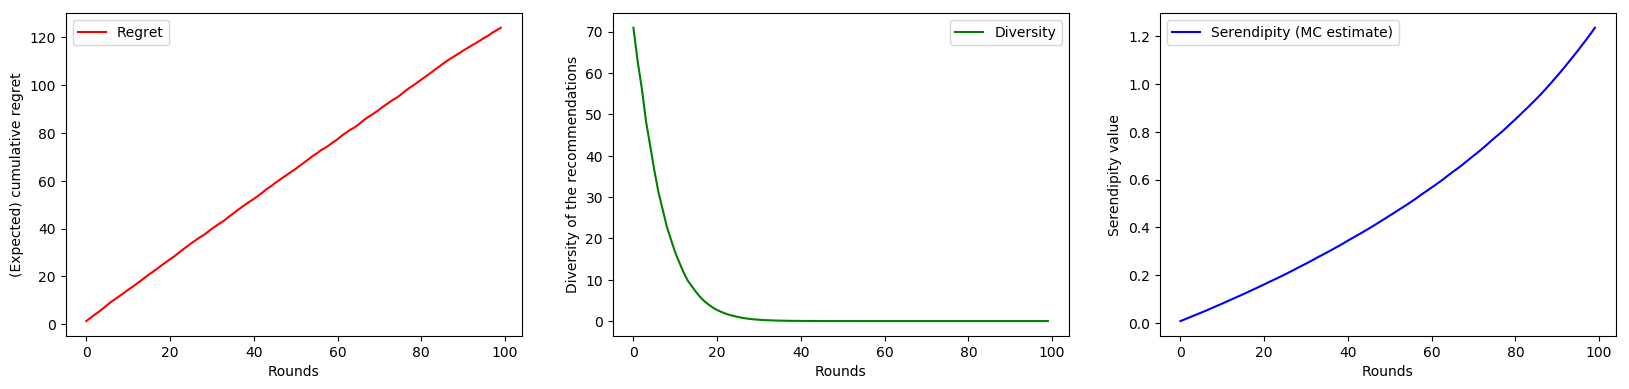
\includegraphics[width=300px]{../../Results/ml-20m/random-48sec.png}
\end{center}
\begin{center}
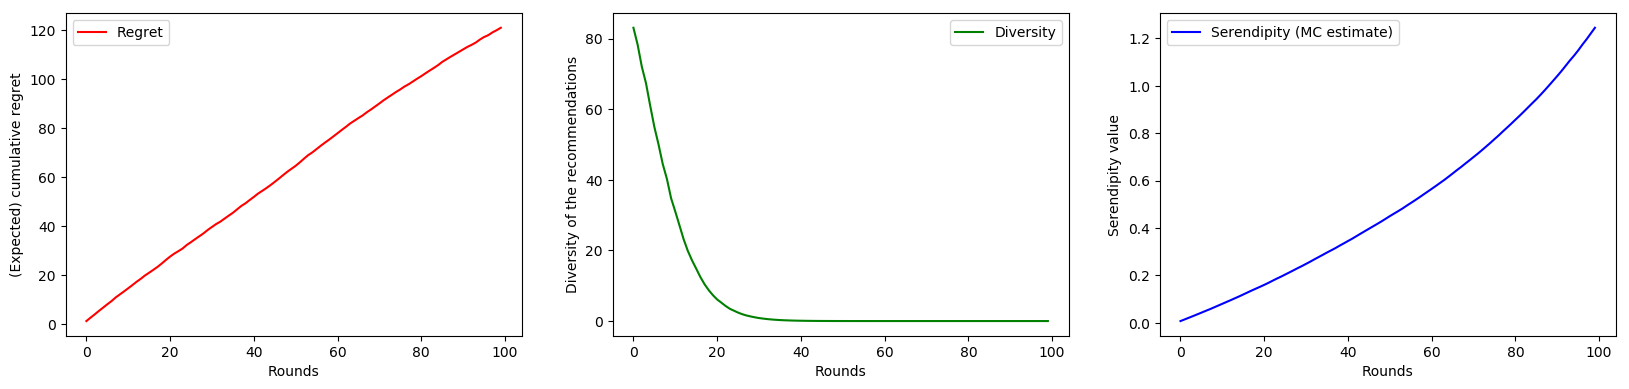
\includegraphics[width=300px]{../../Results/ml-20m/greedy-2min16sec.png}
\end{center}

\end{frame}

\begin{frame}{\textbf{Results} Regret, diversity, serendipity curves}

\textbf{ml-20m} dataset, adapted method (\emph{top}) and LinUCB methods

\begin{center}
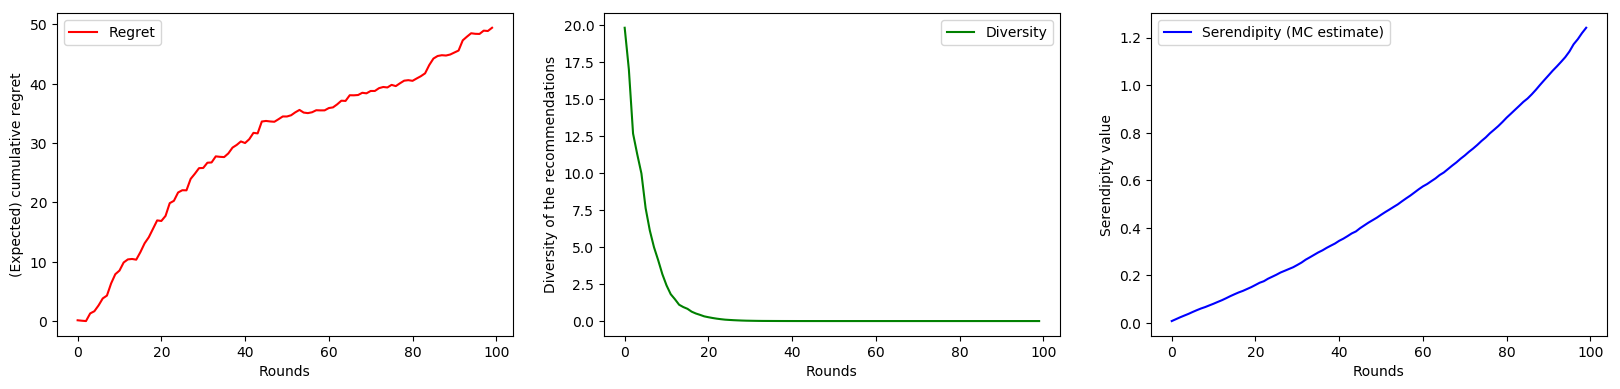
\includegraphics[width=300px]{../../Results/ml-20m/lagree-1min49sec.png}
\end{center}
\begin{center}
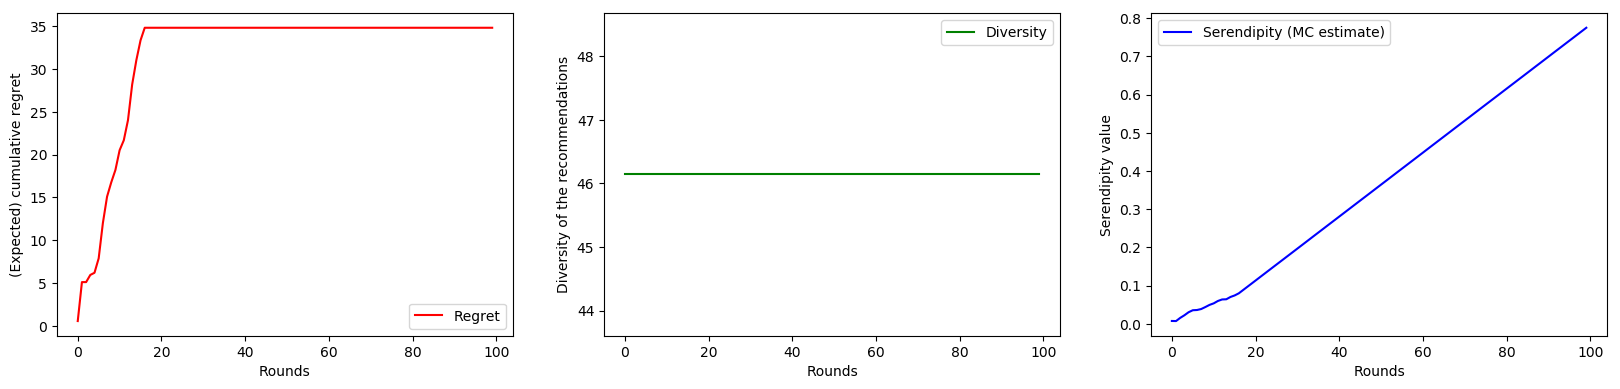
\includegraphics[width=300px]{../../Results/ml-20m/linUCB-53sec.png}
\end{center}

\end{frame}

\subsection{Qualitative Results}

\begin{frame}{\textbf{Results} Variation of parameter $s$}

\begin{center}
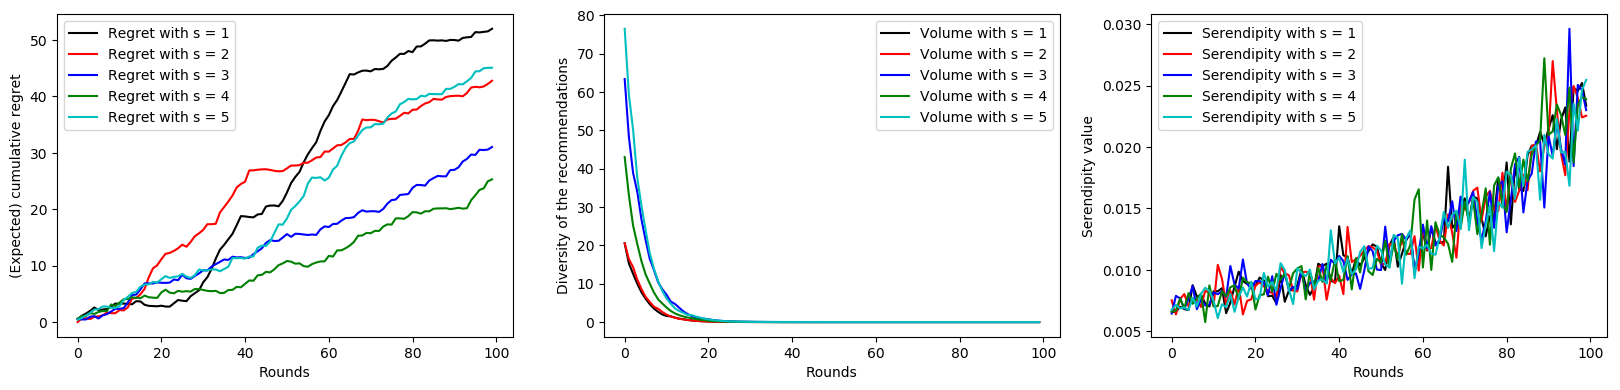
\includegraphics[width=320px]{../../Results/ml-20m/lagree.png}
\end{center}

\textbf{Remarks}:
\begin{itemize}
\item When $s$ increases (up to some point), diversity increases and regret decreases
% which makes sense with respect to the definition of s
\pause
\item From some value of $s$, regret increases again
% diversity-accuracy dilemma
\pause
\item Little influence of $s$ on the (cumulative) serendipity value...
% this is maybe due to the fact that the peaks in the serendipity values are averaged and thus smoothed and there was maybe a better way to show it. I saw it as a "regret" function but we might actually be more interested in the number of peaks in the serendipity value than in the actual values
\end{itemize}

\end{frame}

\section{Conclusion}

 \begin{frame}
 \tableofcontents[currentsection]
 \end{frame}

 \begin{frame}

\begin{block}{Outlook}

\begin{enumerate}
\item A measure for serendipity
\pause
\item A method that tackles the problem of recommendation with serendipity
\pause
\item Benchmark with classic/naive methods of recommendation
\end{enumerate}
\end{block}

\pause 

\begin{alertblock}{What remains to be done}

\begin{itemize}
\item Testing with methods that might be more relevant: Rotting Bandits \cite{seznec2018rotting}, Outside-The-Box recommendation \cite{abbassi2009getting}
\pause
\item User similarity has been ignored here
\pause
\item The parametrization with the serendipity threshold $s$ has an influence on regret and diversity, but not so much on the serendipity measure!! 
% Method should be improved
\end{itemize}
\end{alertblock}

\end{frame}

\begin{frame}[allowframebreaks]{References}
\bibliography{../biblio.bib} 
\bibliographystyle{apalike}
\end{frame}
\end{document}


